\label{chpt:discussion} % for referencing this chapter elsewhere, use \ref{chpt:label}
\lhead{\emph{Discussion}} % This is for the header on each page - perhaps a shortened title

The analysis of this section includes eclipse modelled data from several sources: the 15 systems contained in this thesis, the 15 CVs characterised by \citet{McAllister2019}, and the 14 CVs modelled by \citet{Savoury2011}. An additional 4 systems from \citet{mcallister2015,mcallister2017, mcallister2017b}; and \citet{copperwheat2010} were used, detailed in Table~\ref{appendix:table:supplementary systems}. A full catalogue of all these data is given in Appendix~\ref{appendix:eclipse modelled CV data tables}.
There is some overlap between the data of \citet{McAllister2019} and \citet{Savoury2011}, and where this is the case the more recent findings of \citet{McAllister2019} are preferred.




\section{Inferring mass loss rate from donor properties}
\label{sect:discussion:evolutionary modelling}

First, I compare the mass loss rates of the donor inferred from donor properties, with the mass loss rates inferred from the white dwarf properties. Figure~\ref{fig:discussion:compare Mdot from donor and WD} plots the $\dot M$ from each method, and two differences between the data are immediately obvious: the white dwarf properties consistently indicate a higher $\dot M$, and using the donor properties results in significantly larger uncertainties.

The white dwarf indicating a higher mass loss rate is expected, as recent dwarf novae (a.k.a periods of intense accretion onto the white dwarf) cause the surface to heat up, but after a dwarf nova has subsided the white dwarf will take hundreds to tens of thousands of years to adjust to the lower accretion rate.
Several of the CVs in this sample were identified for eclipse modelling follow-up \textit{explicitly} based on observations of recent outbursts, so it is unsurprising that the white dwarf can indicate $\dot M$ an order of magnitude higher than the donor suggests. As the white dwarf is subject to inflation by these short-term variations, the donor-based method is considered more reliable for the long-term $\dot M$ baseline and hereafter when values of $\dot M$ are used, they are the values derived from the donor properties.
\begin{figure}
    \centering
    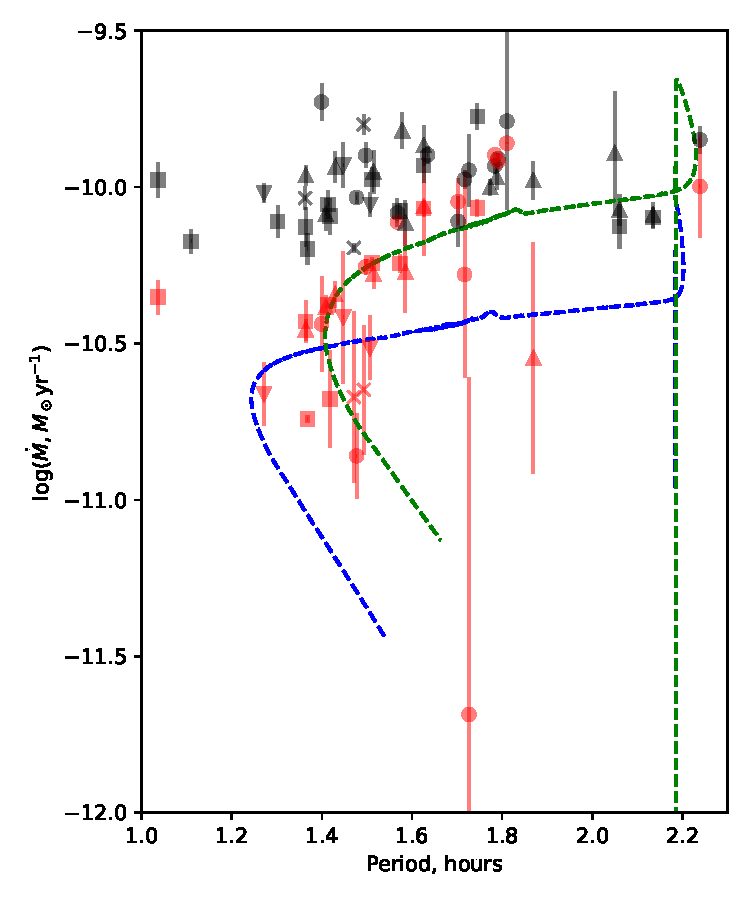
\includegraphics[width=\textwidth]{figures/results/Mdot/compare_mdot_from_donor_vs_wd_vs_period.pdf}
    \caption{Comparing the mass loss rates inferred from the donor properties ({\bf red crosses}) with those inferred from the white dwarf properties ({\bf blue crosses}).}
    \label{fig:discussion:compare Mdot from donor and WD}
\end{figure}


\subsection{Mass loss rate correlations}

Recall from the discussion in \S\ref{sect:introduction:magnetic braking} that, if the missing AML from CV models is rooted in residual magnetic braking, {\it and these prescriptions for magnetism are accurate}, we would expect to see a correlation between $M_{\rm donor}$ and $\dot M$. No such correlation is expected with $M_{\rm wd}$.
This is because both prescriptions are dependent on the Rossby number, a function of the rotational period, which itself is a function of donor mass for short period CVs.
If, however, the eCAML model is correct and the source of the missing AML is the white dwarf's ejecta carrying momentum with it from the system (refer to \S\ref{sect:introduction:CAML}), we would expect a correlation between $M_{\rm wd}$ and $\dot M$.
Of course, the two sources of extra AML are not mutually exclusive, and may co-exist.

To probe for these correlations the $\chi^2$ test is insufficient, since both axes have significant uncertainty. The orthogonal distance between the line and data is again minimised, similar to the previous section.

Figure~\ref{fig:discussion:donor mass vs Mdot fit} shows the best fit line for $\dot M(M_{\rm donor})$, and Figure~\ref{fig:discussion:white dwarf mass vs Mdot fit} is the fit for $\dot M(M_{\rm wd})$.

The correlation between $M_{\rm wd}$ and $\dot M$, is reasonably confident -- the best-fit gradient is $4.5\sigma$ from the null-hypothesis of 0.

However, no correlation is found between $\dot M$ and $M_{\rm donor}$, and Figure~\ref{fig:discussion:donor mass vs Mdot fit} clearly shows an incredibly wide range of gradients to be consistent with the data. If errors are ignored, the data have a Pearson's rank correlation coefficient of

Based on these results, it is unlikely that residual magnetic braking is responsible for the excess AML in CVs, but still possible that the drag imposed by nova material is the cause.
However, there are a few factors to consider when deciding how convincing these findings are.
The sample size is still small, only 25 systems, and the uncertainty in $\dot M$ are large. In addition, there may be a problem with systematic error -- it may that this sample is biased towards CVs with more excess AML, as these would be more inflated and thus less likely to be smaller than the Brown relation suggests for a zero-$\dot M$ star.
A significant source of unreliability is likely to be the mass-radius relationship used to calibrate the donor models. A more robust understanding of the low-mass main sequence mass-radius relation is crucial to a more confident re-analysis of these results.

\begin{figure}
    \centering
    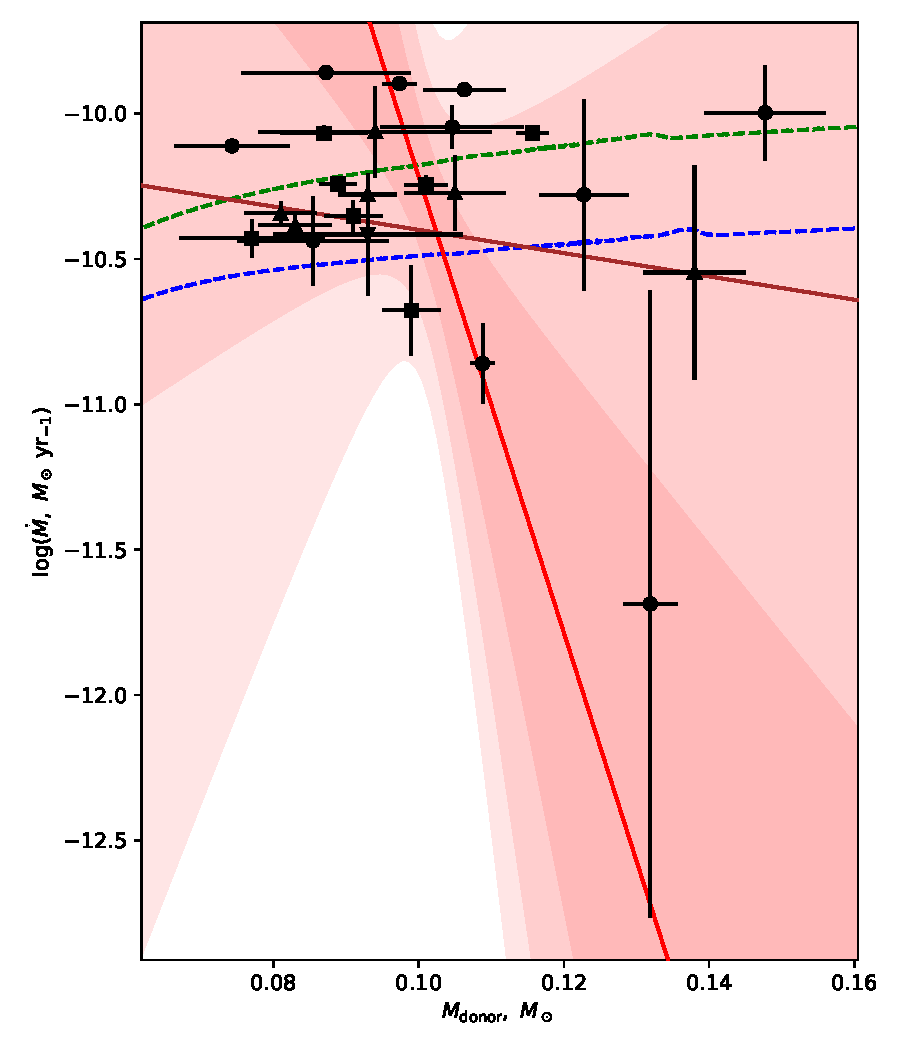
\includegraphics[width=\textwidth]{figures/results/Mdot/Mr_Mdot.pdf}
    \caption{Showing the correlation between the donor mass and mass loss rate. The {\bf black crosses with error bars} show the observations, and the {\bf red line} shows the best fit to the data, with the {\bf shaded red region} showing the coverage of the uncertainty in the line parameters. The darkest region is $1\sigma$, the middle region is $2\sigma$, and the lightest region shows $3\sigma$, and the {\rm brown line} is the initial guess for fitting. The {\bf dashed blue line} shows the value predicted by the `standard' MESA CV model, and the {\bf dashed green line} is the `optimal' MESA CV track. The best fit line has the form $\log (\dot M,\ M_\odot\ {\rm yr}^{-1}) = (-79\pm48) (M_{\rm donor}, M_\odot) - (2.3\pm4.9)$. }
    \label{fig:discussion:donor mass vs Mdot fit}
\end{figure}
% \begin{figure}
%     \centering
%     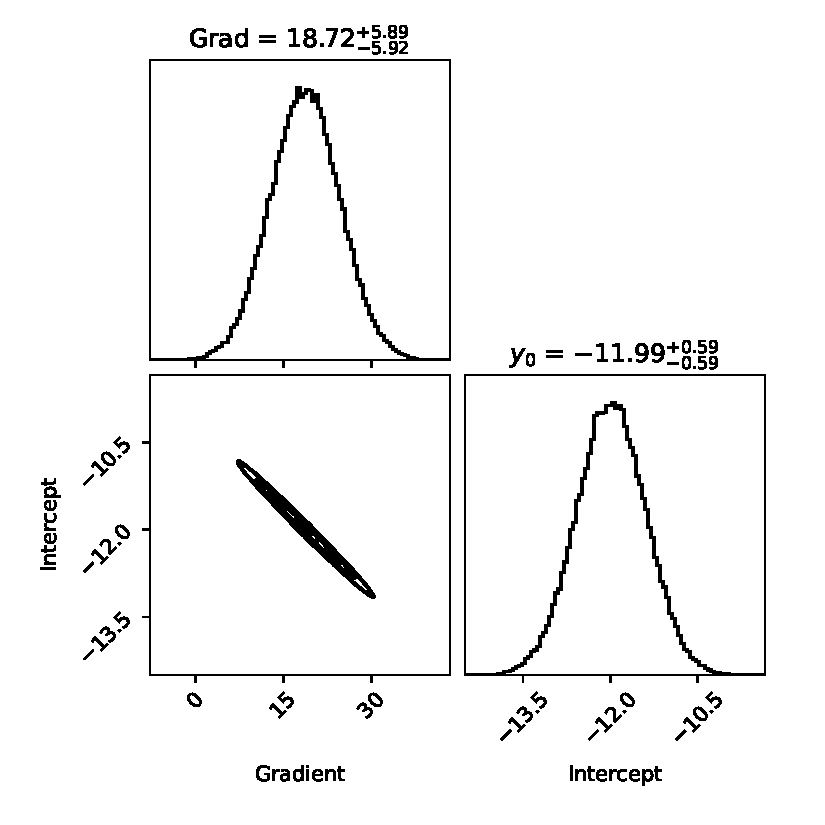
\includegraphics[width=\textwidth]{figures/results/Mdot/Mr_Mdot_corner.pdf}
%     \caption{Showing the posterior distributions of the gradient and intercept of the best fit line in Figure~\ref{fig:discussion:donor mass vs Mdot fit}.}
%     \label{fig:discussion:donor mass vs Mdot corner}
% \end{figure}
\begin{figure}
    \centering
    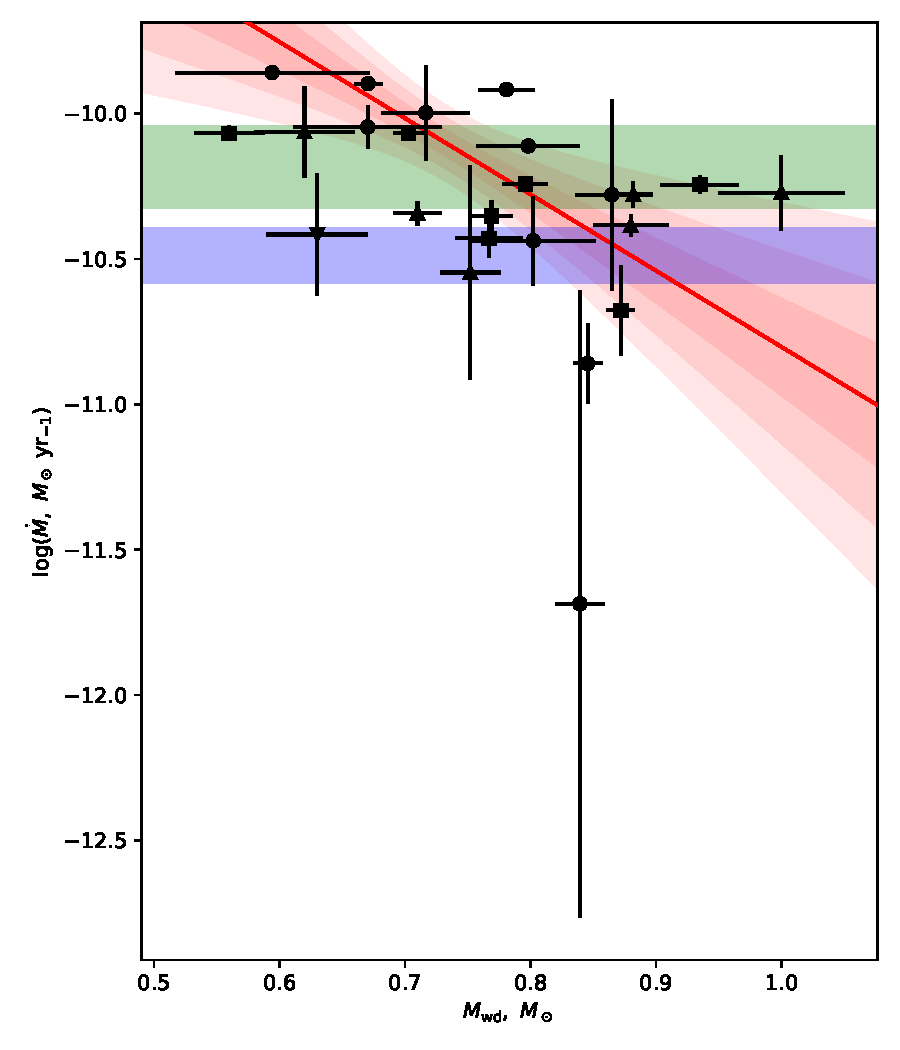
\includegraphics[width=\textwidth]{figures/results/Mdot/Mwd_Mdot.pdf}
    \caption{Showing the correlation between the white dwarf mass and mass loss rate. Symbols are similar to Figure~\ref{fig:discussion:donor mass vs Mdot fit}, though here the range of values predicted by the `standard' and `optimal' MESA CV models are shown as the {\bf blue shaded region} and {\bf green shaded region}, respectively. The best fit line has the form $\log ( \dot M,\ M_\odot\ {\rm yr}^{-1}) = (-2.62 \pm 0.60) (M_{\rm wd}, M_\odot) - (8.18 \pm 0.44)$}
    \label{fig:discussion:white dwarf mass vs Mdot fit}
\end{figure}
% \begin{figure}
%     \centering
%     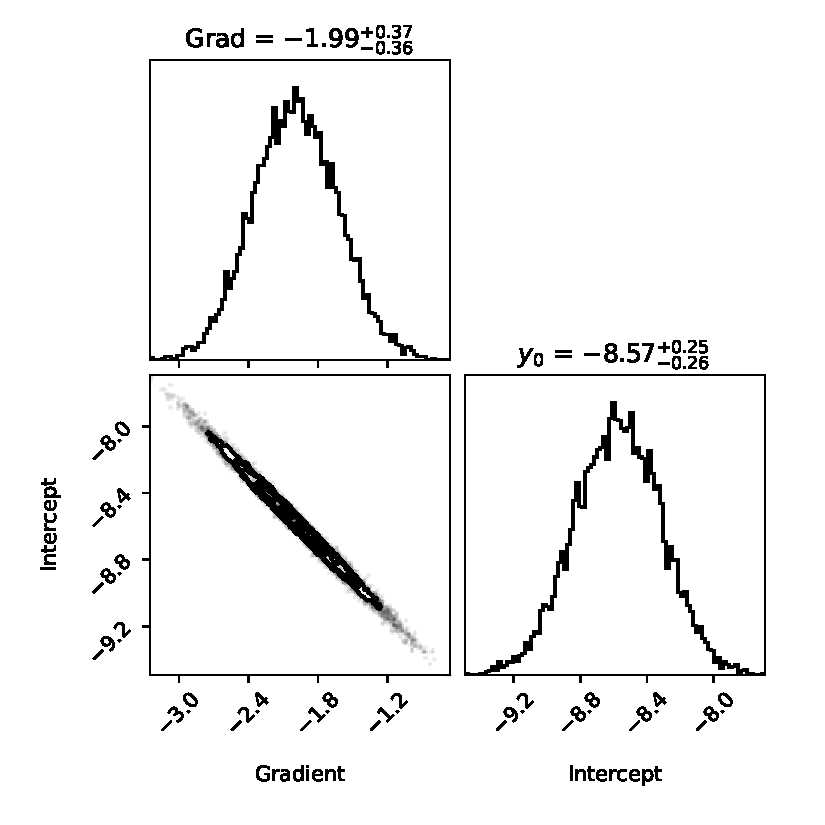
\includegraphics[width=\textwidth]{figures/results/Mdot/Mwd_Mdot_corner.pdf}
%     \caption{Showing the posterior distributions of the gradient and intercept of the best fit line in Figure~\ref{fig:discussion:white dwarf mass vs Mdot fit}.}
%     \label{fig:discussion:white dwarf mass vs Mdot corner}
% \end{figure}


\subsection{Measured excess angular momentum loss}

It is possible to more directly probe the AML of the CVs -- Equation~\ref{eqn:modelling:Jdot from Mdot} shows how the AML can be calculated from $M_{\rm wd},\ M_{\rm donor},\ \dot M$, and $a$.
Figures~\ref{fig:discussion:donor mass vs Jdot fit}~and~\ref{fig:discussion:white dwarf mass vs Jdot fit} show the best-fit to the $\dot J$ \textit{excess}, which has had the $\dot J_{\rm GR}$ predicted by MESA at the appropriate donor mass ($\dot J_{\rm MESA}$) subtracted.
Here, the white dwarf mass shows a reasonably confident correlation with the observed $\dot J$ excess, but with large scatter about the best-fit relationship. Similarly to the case of $\dot M$, fitting was unable to find a correlation between $M_{\rm donor}$ and $\dot J$ excess.

\begin{figure}
    \centering
    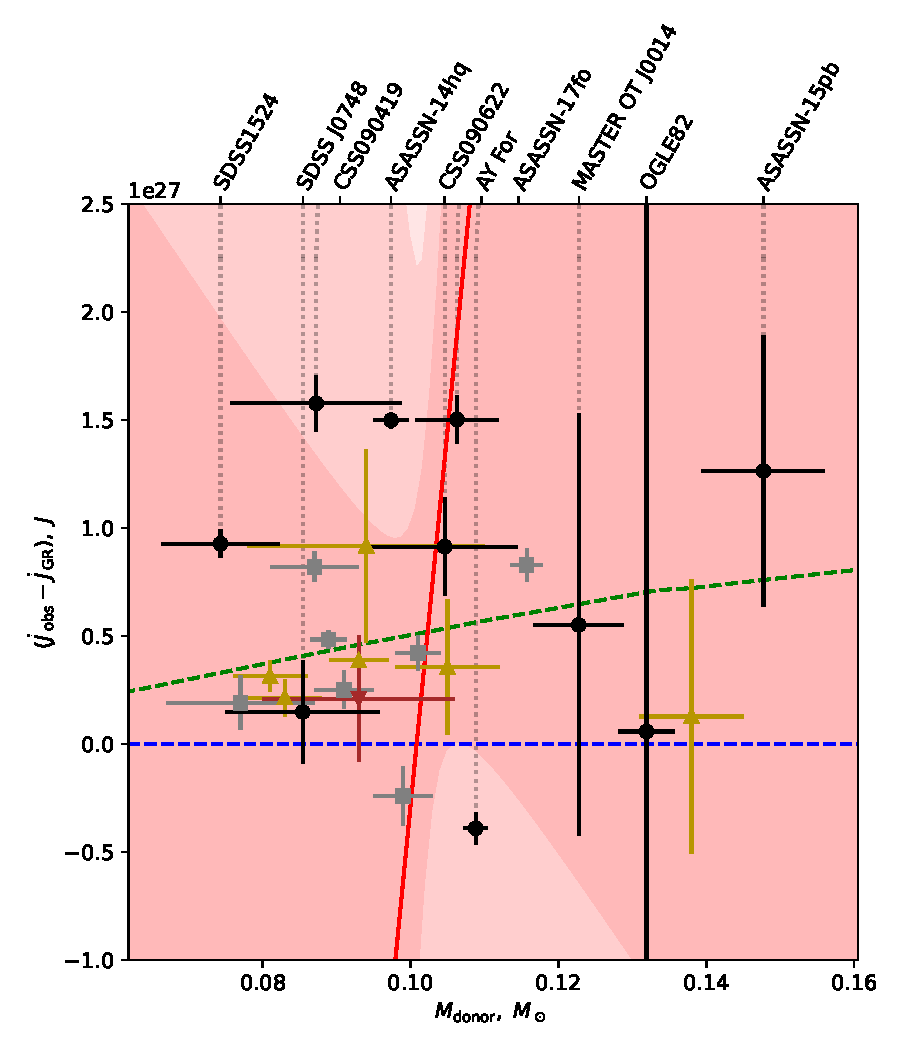
\includegraphics[width=\textwidth]{figures/results/Mdot/Mr_Jdot_ex.pdf}
    \caption{Showing the correlation between the donor mass and angular momentum loss rate, $\dot J$. Symbols are similar to Figure~\ref{fig:discussion:donor mass vs Mdot fit}, though here the {\bf dashed blue line} shows perfect agreement between observations and gravitational angular momentum loss. Note that the datum with vertical errors spanning the full height of the plot extend by approximately an order of magnitude in each direction, but are truncated for clarity. The line of best fit has the form $(\dot J_{\rm obs} - \dot J_{\rm MESA}), J = (5\pm10) \times 10^{29}(M_{\rm donor}, M_\odot) - (5\pm10)\times10^{28}$}
    \label{fig:discussion:donor mass vs Jdot fit}
\end{figure}
% \begin{figure}
%     \centering
%     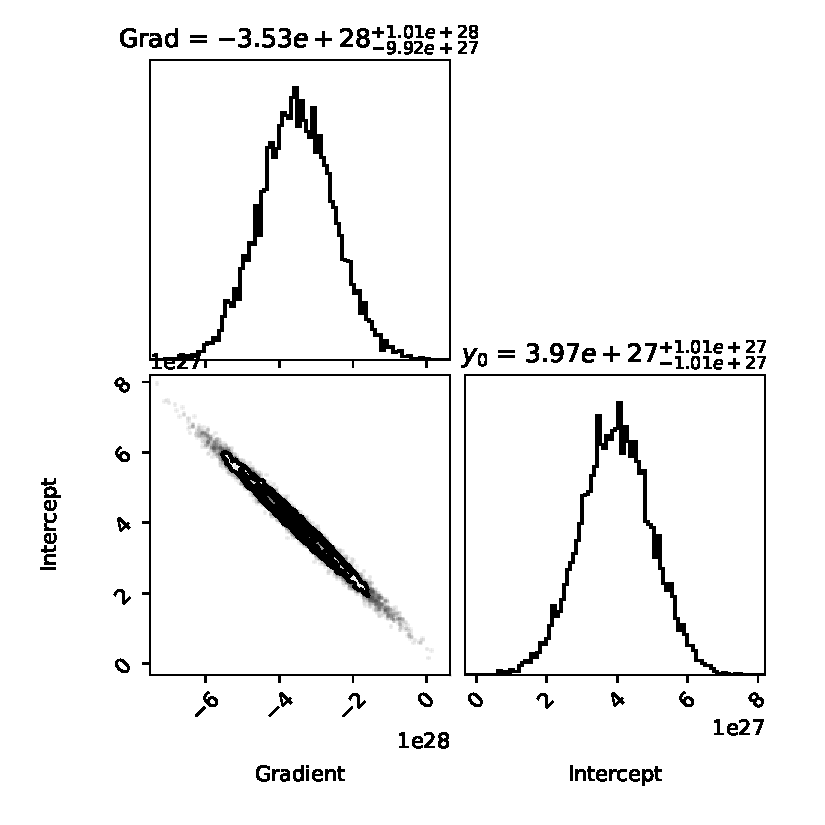
\includegraphics[width=\textwidth]{figures/results/Mdot/Mr_Jdot_ex_corner.pdf}
%     \caption{Showing the posterior distributions of the gradient and intercept of the best fit line in Figure~\ref{fig:discussion:donor mass vs Jdot fit}.}
%     \label{fig:discussion:donor mass vs Jdot corner}
% \end{figure}

\begin{figure}
    \centering
    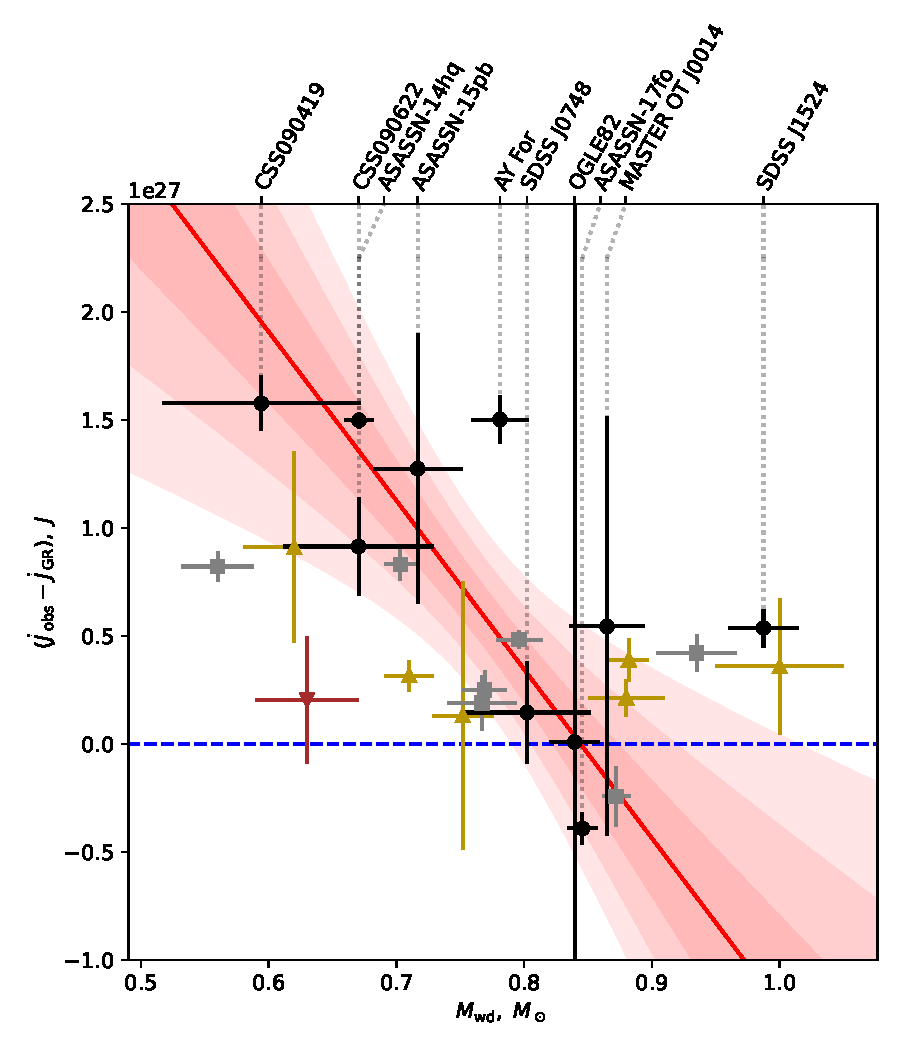
\includegraphics[width=\textwidth]{figures/results/Mdot/Mwd_Jdot_ex.pdf}
    \caption{Showing the correlation between the white dwarf mass and angular momentum loss rate, $\dot J$. Symbols are similar to Figure~\ref{fig:discussion:white dwarf mass vs Jdot fit}, and the best fit line has the form $(\dot J_{\rm obs} - \dot J_{\rm MESA}), J = -5.7\pm1.3) \times 10^{27}(M_{\rm wd}, M_\odot) - (4.6\pm0.96)\times10^{26}$}
    \label{fig:discussion:white dwarf mass vs Jdot fit}
\end{figure}
% \begin{figure}
%     \centering
%     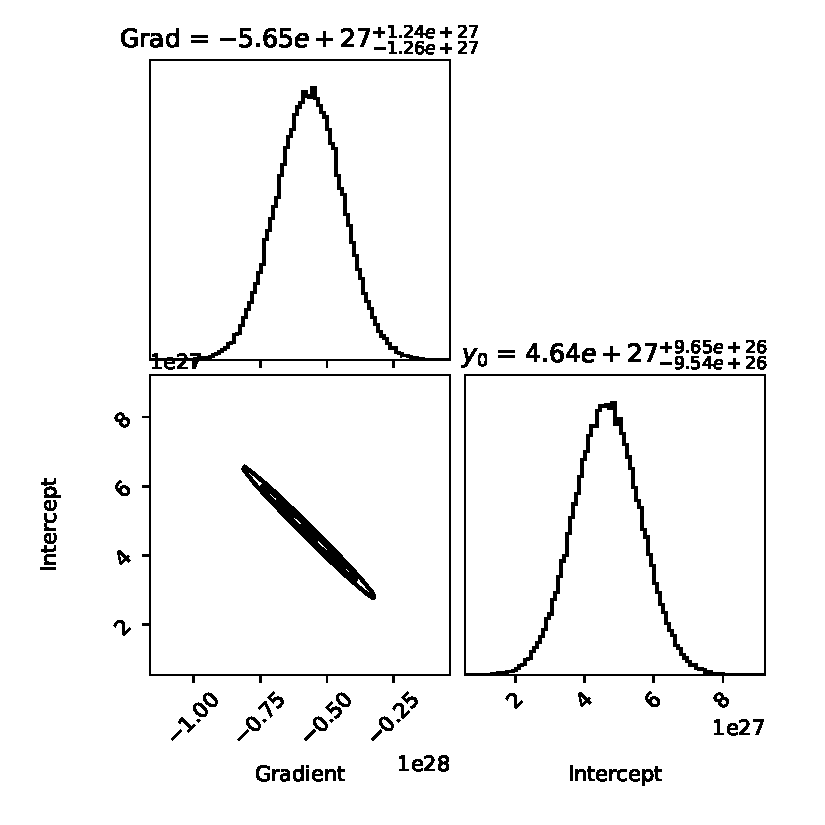
\includegraphics[width=\textwidth]{figures/results/Mdot/Mwd_Jdot_ex_corner.pdf}
%     \caption{Showing the posterior distributions of the gradient and intercept of the best fit line in Figure~\ref{fig:discussion:white dwarf mass vs Jdot fit}.}
%     \label{fig:discussion:white dwarf mass vs Jdot corner}
% \end{figure}


Three possibilities for the form of excess AML were suggested in \S\ref{sect:discussion AML}: the excess AML also declines in strength but more slowly than gravitational losses; excess AML is roughly constant across the range of $M_{\rm donor}$ or $M_{\rm donor}$; or excess AML increases in strength towards lower $M_{\rm donor}$ or $M_{\rm wd}$.
We can now see that the excess AML appears to increase in strength towards lower $M_{\rm wd}$.

% Based on the analysis above, it appears that eCAML is the better model for the excess AML of a short period CV, with there being consistent signs of increasing excess AML towards both lower donor masses, and lower white dwarf masses.
% We can now discriminate between these with the quantitative analysis given here, and see that the degree of excess AML is most likely to be a negative correlation with $M_{\rm wd}$, in line with the CAML model of CVs.


Recall from \S\ref{sect:introduction:CAML} that under eCAML, the efficiency parameter $\nu$, is given by $C/M_{\rm wd}$, and typical values of $C$ are roughly chosen to be $0.3 - 0.4$, to reproduce the observed CV population distribution.
\begin{equation}
    \label{eqn:ecaml general}
    \frac{\dot J_{CAML}}{J} = \nu \frac{\dot M_{\rm donor}}{M_{\rm donor}}
\end{equation}
Assuming that eCAML is the sole source of excess AML, we can now measure a value of $\nu$. To do this, I use a slightly modified version of Equation~\ref{eqn:ecaml general}, which accounts for the choice of the form of $\nu$;
\begin{equation}
    \frac{\dot J_{CAML}}{J} = C \frac{\dot M_{\rm donor}}{M_{\rm donor} M_{\rm wd}}
\end{equation}
$C$ can then be fit to data, again minimising the orthogonal distance to the data, though this fit is limited to the subset of the observations for which $\dot M$ could be determined.
Doing so finds a best-fit $C = 0.32 \pm0.05$ with impressively good agreement between the model and data, shown in Figure~\ref{fig:discussion:calibrating ecaml relationship}. This value of $C$ is also remarkably close to that estimated by \citet{Schreiber2016}. \todo{This is the wrong one! I need the one with no y-intercept.}
\begin{figure}
    \centering
    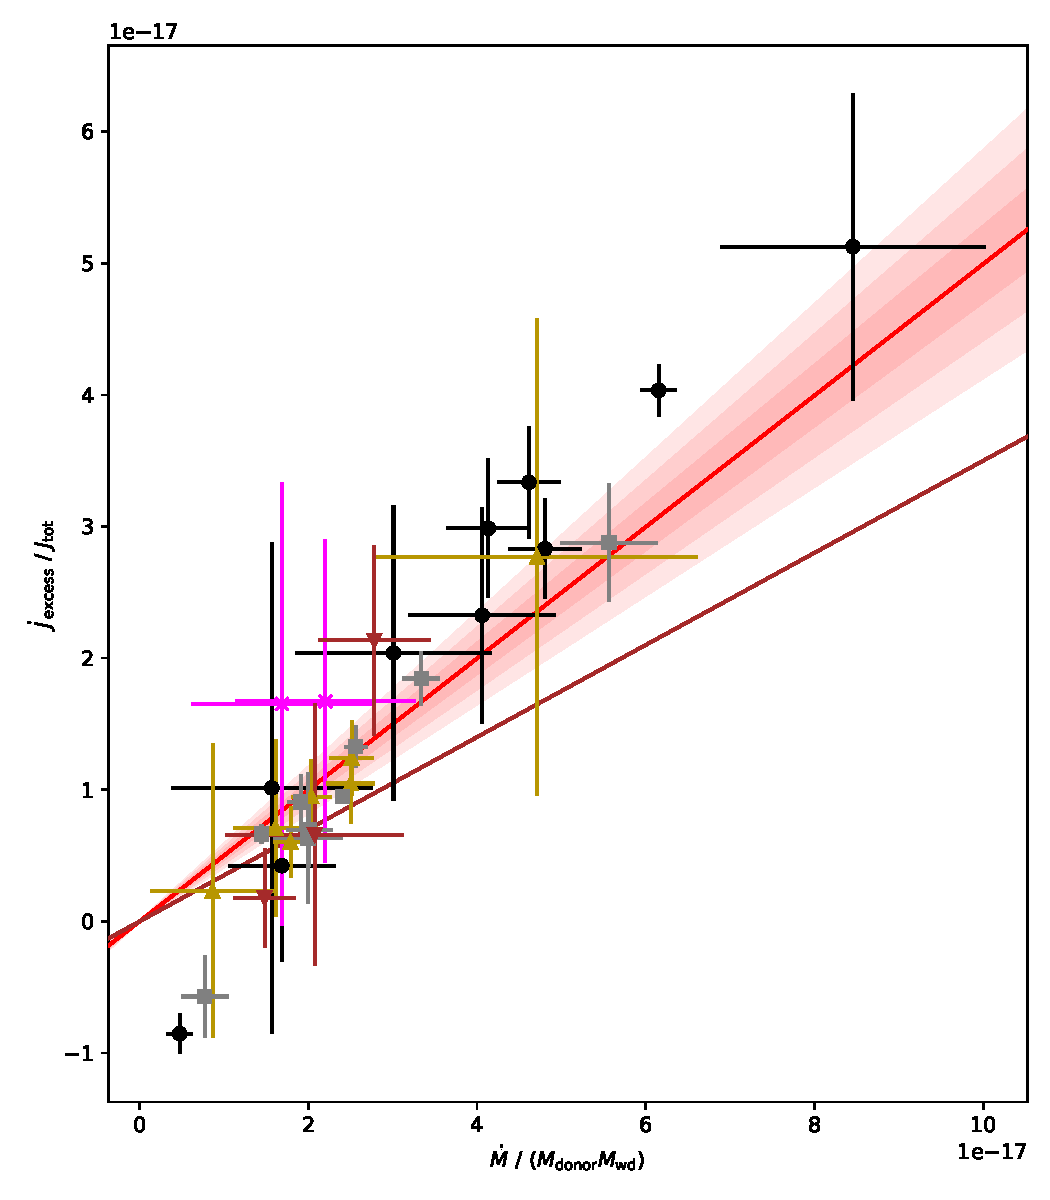
\includegraphics[width=\textwidth]{figures/results/Mdot/eCAML_nu_no_intercept_fit.pdf}
    \caption{DO THIS CAPTION}
    \label{fig:discussion:calibrating ecaml relationship}
\end{figure}

As a final test of eCAML, the stability plot given in Figure~\ref{fig:introduction:Schreiber 2016 figure 2} can be augmented to include the new CVs of this work, and the best-fit value of $\nu$.\todo{Fix the label!}
This is shown in Figure~\ref{fig:discussion:calibrated eCAML}, from which we can see that no low $M_{\rm donor}$ CVs exist outside the stability region demanded by the newly calibrated eCAML.
\begin{figure}
    \centering
    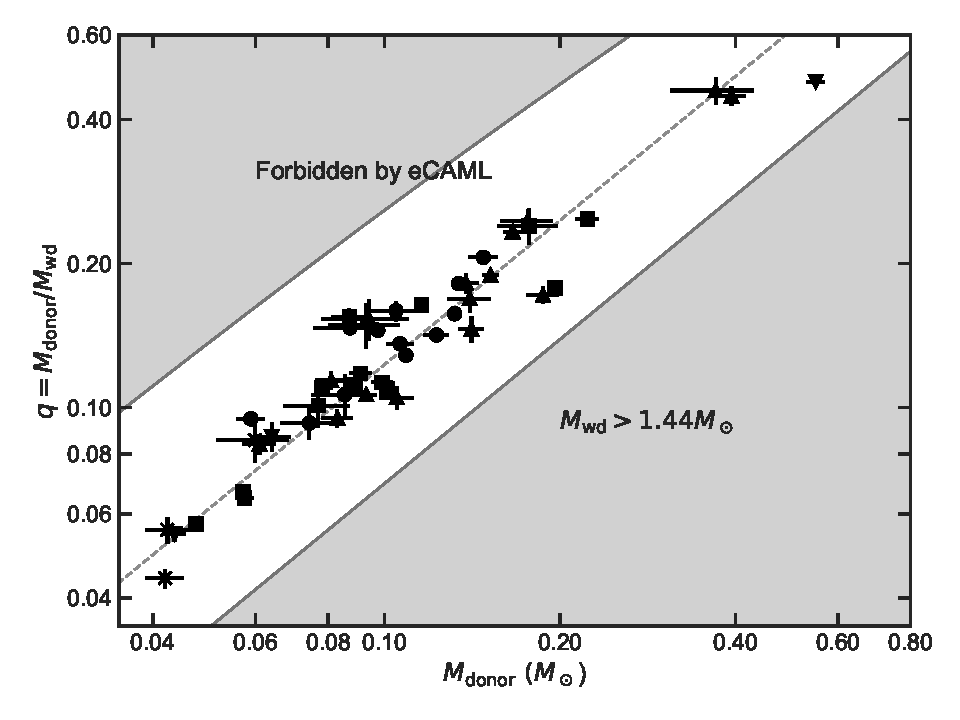
\includegraphics[width=\textwidth]{figures/results/Mdot/ecaml_nointercept.pdf}
    \caption{Showing the distribution of eclipse modelled, low $M_{\rm donor}$ CVs compared to the region of stability demanded by eCAML. The {\bf shaded grey regions} are forbidden, either because the white dwarf exceeds the Chandrasekhar limit (lower region), or because mass transfer becomes dynamically unstable (upper region). The {\bf dashed line} shows the mass ratio that a CV would have with $M_{\rm wd} = 0.81 M_\odot$. Data symbology is similar to Figure~\ref{fig:discussion:donor model with eclipsers plotted}}
    \label{fig:discussion:calibrated eCAML}
\end{figure}
These findings underline the success of eCAML in describing CV evolution, but must still be treated with caution. It cannot be ignored that whilst this form of $\nu$ is loosely physically motivated, a less empirical model is highly desirable.
Further, the data clearly suggest that $\frac{\dot J_{CAML}}{J} \neq 0$ at $\dot M = 0$, in direct contradiction with the original formulation. \todo{Talk to Stu about this when he's back. I reckon some algebra is needed to re-derive the stability criterion to allow for this... But it's not physical! How could CAML inhibit AML???}

Further work is needed to grow the population of eclipse modelled low-$M_{\rm donor}$ CVs and improve these statistics, and continued eclipse modelling targeting short period CVs will be valuable to determining the probable source of excess AML.
Specific effort should be targeted towards confident characterisation of CVs at higher $M_{\rm donor}$ of $\sim0.15$, where existing data have large error bars. The clustering of confident data at lower masses leaves the current sample prone to poor extrapolation beyond $\sim 0.11 M_\odot$.
However, lending credence to these results is the consistency with findings of \citet{Pala2021}, who used the white dwarf properties to arrive at a similar conclusion.

\todo{Augment MESA to include my new AML prescription, and run it?}